\chapter{Experimentación}

En este capítulo se expone la experimentación realizada para la evaluación del agente propuesto.

Se empieza ofreciendo los detalles de la experimentación, centrándose en los parámetros utilizados y los experimentos a realizar. Tras esto, se muestran los resultados obtenidos por las dos familias de agentes propuestas (estándares y priorizadas), mostrando además los experimentos que llevaron a la elección del conjunto de datos. Finalmente, se realiza una comparativa de los mejores agentes de cada familia, comparando su rendimiento durante el entrenamiento y al enfrentarse a problemas nuevos, analizando los resultados obtenidos.

\section{Detalles de la experimentación}

En esta sección se describen los principales detalles de la experimentación: los \textbf{parámetros} a utilizar durante los experimentos, las \textbf{métricas} a medir y los \textbf{experimentos} que se ha optado por realizar.

\subsection{Parámetros generales utilizados}

Si bien hay algunos parámetros que varían entre experimentos, la gran mayoría de éstos son reutilizados por toda la experimentación. Para facilitar la reproducibilidad, estos parámetros serán descritos a continuación, mostrando sus valores y su significado.

Los parámetros utilizados y su origen se pueden observar en las siguientes tablas:
\begin{itemize}
	\item Parámetros usados por \textit{Deep Q-Learning} en el Cuadro \ref{tab:dqlparam}.
	
	Los parámetros están basados en los parámetros originales propuestos por DeepMind en su artículo original \cite{Mnih2015HumanlevelCT}, ajustados experimentalmente para adaptarse al problema.
	
	\item Parámetros usados durante el preprocesamiento de imágenes en el Cuadro \ref{tab:imageparam}.
	
	Los parámetros se han elegido manualmente mediante experimentación para ajustarse a las necesidades del problema.
	
	\item Parámetros usados durante la generación de las recompensas en el Cuadro \ref{tab:rewardparam}.
	
	Los parámetros están basados en los parámetros originales propuestos por Carlos Sampedro \textit{et al.} en su trabajo original \cite{Sampedro2018}, adaptándose de forma experimental a las necesidades del proyecto.
\end{itemize}

\begin{table}[h]
\centering
\resizebox{\textwidth}{!}{%
\begin{tabular}{@{}lll@{}}
\toprule
Hiperparámetro                                                                       & Valor & Descripción                                                                                                                                                      \\ \midrule
seed                                                                                 & 0     & Semilla usada para los experimentos                                                                                                                              \\
learning\_rate                                                                       & 0.001 & Ratio de aprendizaje de la red neuronal                                                                                                                          \\
gamma ($\gamma$)                                                                     & 0.99  & Ratio de aprendizaje de DQL                                                                                                                                      \\
epsilon ($\epsilon$)                                                                 & 1.00  & Probabilidad inicial de realizar una acción aleatoria                                                                                                            \\
min\_epsilon ($\epsilon_{min}$)                                                      & 0.05  & \begin{tabular}[c]{@{}l@{}}Probabilidad final de realizar una acción aleatoria\\ (tras min\_epsilon\_percentage episodios)\end{tabular}                          \\
\begin{tabular}[c]{@{}l@{}}min\_epsilon\_percentage \\ ($min\_epsilon$)\end{tabular} & 0.8   & \begin{tabular}[c]{@{}l@{}}Porcentaje de episodios tras el cual epsilon alcanza min\_epsilon\\ (tras el 80\% de los episodios alcanza min\_epsilon)\end{tabular} \\ \bottomrule
\end{tabular}%
}
\caption{Parámetros generales de \textit{Deep Q-Learning.}}
\label{tab:dqlparam}
\end{table}

\begin{table}[h]
\centering
\resizebox{\textwidth}{!}{%
\begin{tabular}{@{}lll@{}}
\toprule
Hiperparámetro      & Valor & Descripción                                                                                                                                                                          \\ \midrule
trim                & 35    & \begin{tabular}[c]{@{}l@{}}Número de píxeles recortados a la imagen por los\\ extremos inferior y superior\end{tabular}                                                              \\
obstacle\_threshold & 0.15  & \begin{tabular}[c]{@{}l@{}}Umbral en la cámara de profundidad a partir del cual\\ se consideran obstáculos\\ (los objetos a menos de obstacle\_threshold son obstáculos)\end{tabular} \\
min\_contour\_area  & 250   & \begin{tabular}[c]{@{}l@{}}Área mínima (en píxeles) de un contorno \\ para ser considerado obstáculo\end{tabular}                                                                    \\ \bottomrule
\end{tabular}%
}
\caption{Parámetros generales del procesamiento de imágenes.}
\label{tab:imageparam}
\end{table}

\begin{table}[h]
\centering
\resizebox{\textwidth}{!}{%
\begin{tabular}{@{}lll@{}}
\toprule
Hiperparámetro                                                                     & Valor & Descripción                                                                                                                                                                                                      \\ \midrule
obstacle\_distance ($l_{max}$)                                                     & 2     & \begin{tabular}[c]{@{}l@{}}Distancia aproximada (en metros) a la que se encuentra un\\ obstáculo en el umbral de detección\end{tabular}                                                                          \\
attraction\_gain ($\alpha$)                                                        & 100   & Ganancia aplicada a la fuerza atractora para aumentar su influencia                                                                                                                                              \\
repulsive\_gain ($\beta$)                                                          & 15    & Ganancia aplicada a la fuerza repulsiva para aumentar su influencia                                                                                                                                              \\
repulsive\_limit ($k$)                                                             & 0.04  & Valor usado para limitar la influencia de la fuerza repulsiva                                                                                                                                                    \\
\begin{tabular}[c]{@{}l@{}}repulsive\_goal\_influence \\ ($d_{infl}$)\end{tabular} & 0.75  & \begin{tabular}[c]{@{}l@{}}Porcentaje usado para limitar la influencia de la fuerza repulsiva\\ Si la distancia a la meta es menor que $l_{max} * d_{infl}$,\\ la fuerza repulsiva se ve disminuida\end{tabular} \\
success\_reward                                                                    & 10    & Recompensa por un episodio con éxito                                                                                                                                                                             \\
failure\_penalty                                                                   & -100  & Penalización por un episodio fallido o una colisión                                                                                                                                                              \\ \bottomrule
\end{tabular}%
}
\caption{Parámetros generales de la generación de recompensas.}
\label{tab:rewardparam}
\end{table}

Los parámetros específicos usados por cada experimento serán detallados durante la definición de los experimentos a realizar. La lista concreta y completa de los parámetros de cada experimento está disponible en el fichero de configuración correspondiente.

\subsection{Experimentos realizados}

Se ha optado por realizar un total de \textbf{ocho} experimentos, diviendo estos experimentos en dos grandes grupos:

\begin{itemize}
	\item \textbf{Entrenamiento de agentes estándares:} Estos experimentos consisten en el entrenamiento de agentes utilizando una versión estándar de \textbf{Deep Q-Learning} (sin ninguna de las mejoras propuestas) durante un total de \textbf{15000} episodios. Estos agentes cuentan con un \textit{Replay Memory} de \textbf{20000} entradas, usando muestras de \textbf{64} experiencias por entrenamiento.
	
	Especificamente, se han entrenado las siguientes combinaciones de parámetros:
	\begin{itemize}
		\item Recompensa de contornos / Sin colisiones.
		\item Recompensa de contornos / Con colisiones.
		\item Recompensa de columnas (8 columnas) / Sin colisiones.
		\item Recompensa de columnas (8 columnas) / Con colisiones.
	\end{itemize}
	
	\item \textbf{Entrenamiento de agentes priorizados:} Estos experimentos consisten en el entrenamiento de agentes utilizando \textbf{Deep Q-Learning} con \textbf{Prioritized Experience Replay} (muestreando las experiencias con más error) durante un total de \textbf{3000} episodios. Estos agentes cuentan con un \textit{Replay Memory} de \textbf{5000} entradas, usando muestras de \textbf{32} experiencias por entrenamiento. Además, \textit{Prioritized Experience Replay} utiliza parámetros $\alpha = 0.5$ y $\beta = 0.5$.
	
	Especificamente, se han entrenado las siguientes combinaciones de parámetros:
	\begin{itemize}
		\item Recompensa de contornos / Sin colisiones.
		\item Recompensa de contornos / Con colisiones.
		\item Recompensa de columnas (8 columnas) / Sin colisiones.
		\item Recompensa de columnas (8 columnas) / Con colisiones.
	\end{itemize}
	
	El motivo de que el entrenamiento de estos agentes haya sido más corto y limitado (a nivel de tamaño del \textit{Replay Memory}) es las limitaciones en la capacidad computacional disponible durante el entrenamiento. El algoritmo es notablemente más lento y requiere una mayor cantidad de memoria, por lo que fue necesario reducir la envergadura de los experimentos para permitir acabarlos en un tiempo razonable. 
\end{itemize}

Tras la experimentación de ambos grupos, se realizan comparaciones del rendimiento de los dos mejores agentes de cada grupo durante \textbf{3000} episodios, para compararlos en condiciones de igualdad. Finalmente, se comparará el rendimiento de todos los agentes junto a varios \textit{benchmarks} ofrecidos por \textit{Habitat} (incluyendo varios agentes aleatorios y heurísticos y un agente implementando \textit{Proximal Policy Optimization}) para estudiar el rendimiento de cada agente al enfrentarse a problemas reales.

Todos los experimentos han sido realizados usando el conjunto de datos \textit{Gibson}, al ser éste considerado un conjunto de datos más simple que \textit{Matterport3D} \cite{habitat19iccv}. Además, se ha realizado una experimentación breve (detallada en la próxima sección) que apoya esta decisión.

\subsection{Gráficos generados durante el entrenamiento}

Como ya se mencionó en el capítulo anterior, el proceso de entrenamiento del agente almacena las siguientes métricas en un fichero de \textit{log} al final de cada episodio:
\begin{itemize}
	\item Número del episodio.
	\item Duración del episodio (en segundos).
	\item Número de acciones realizadas durante el episodio.
	\item Distancia inicial y final hasta la meta.
	\item Distancia recorrida hasta la meta ($dist\_inicial - dist\_final$).
	\item Exitoso (\textbf{Verdadero} si el agente ha alcanzado la meta, \textbf{Falso} en cualquier otro caso).
	\item Recompensa media obtenida.
\end{itemize}

Ahora bien, no todas estas métricas son comparables de forma honesta. Por ejemplo, al tener cada episodio una distancia inicial distinta, la distancia recorrida no se puede comparar de forma directa. Por tanto, se ha optado por transformar algunas de las métricas para poder realizar una comparación más justa, generando los siguientes \textbf{gráficos} durante el entrenamiento:
\begin{itemize}
	\item Diagrama de líneas de la \textbf{duración cumulativa por episodio} (en segundos).
	\item Diagrama de líneas de las acciones realizadas por episodio.
	\item Diagrama de líneas del \textbf{porcentaje de distancia recorrido} hasta la meta.
	
	Este porcentaje, en el rango $[0.0, 1.0]$, indica el porcentaje total de distancia recorrido desde la posición inicial hasta la meta. Como ejemplo, un agente con distancia inicial de $10$ metros y distancia final de $5$ metros tendría un porcentaje de $0.5$.
	
	Se utiliza un porcentaje para normalizar la distancia recorrida por cada agente, cambiando la unidad de metros (no indicativa debido a la variabilidad en la longitud total de los episodios) a un porcentaje indicando la cantidad de episodio completada.
	\item Diagrama de líneas de recompensa media por episodio.
	\item Diagrama de barras del \textbf{número total de episodios completados con éxito}.
	
	Este diagrama permite comparar el rendimiento de los agentes de forma más simple que intentar interpretar el diagrama de distancias para observar los episodios completados.
\end{itemize}

Todos los diagramas de líneas han sido \textbf{suavizados} usando como datos la \textbf{media de los valores de los últimos 50 episodios}. De esta forma se reduce notablemente el ruido en las gráficas (haciendolos más legibles) sin perder la información recogida en éstos.

\subsection{Métricas usadas durante la evaluación}

Para la evaluación del rendimiento de los agentes entrenados, se mide el valor medio de las siguientes métricas durante \textbf{100} episodios en entornos no usados durante el entrenamiento:
\begin{itemize}
	\item Distancia a la meta (en metros).
	\item Tasa de éxito.
	\item \textit{Success weighted by Path Length (SPL)}.
	\item \textit{SPL} suavizado.
	\item Número de colisiones.
\end{itemize}

Además, se ofrecen vídeos mostrando el rendimiento de los agentes en los entornos, para poder observar de forma directa el comportamiento de los agentes entrenados.

\section{Resultados obtenidos}

En esta sección se muestran los resultados obtenidos para cada grupo de experimentos mencionado previamente. Además, se muestra un breve análisis de los resultados que propiciaron elegir \textit{Gibson} como conjunto de datos.

\subsection{Elección del conjunto de datos}

Para estudiar la elección del conjunto de datos, se ha comparado el rendimiento de dos agentes equivalentes (\textit{Deep Q-Learning} básico sin colisiones con recompensas de contornos) durante \textbf{15000} episodios de entrenamiento, con especial interés en los episodios completados con éxito y la distancia recorrida hasta la meta.

Como se puede ver inmediatamente en la Figura \ref{fig:chap6-dataset-success}, el agente entrenado usando \textit{Gibson} es capaz de completar una cantidad de episodios notablemente superior a la de su equivalente entrenado con \textit{Matterport3D}. Concretamente, el agente de \textit{Gibson} completa con éxito aproximadamente \textbf{160 episodios} - alrededor de cuatro veces más episodios que el agente de \textit{Matterport3D}, completando \textbf{40 episodios}.

\begin{figure}[h]
    \centering
    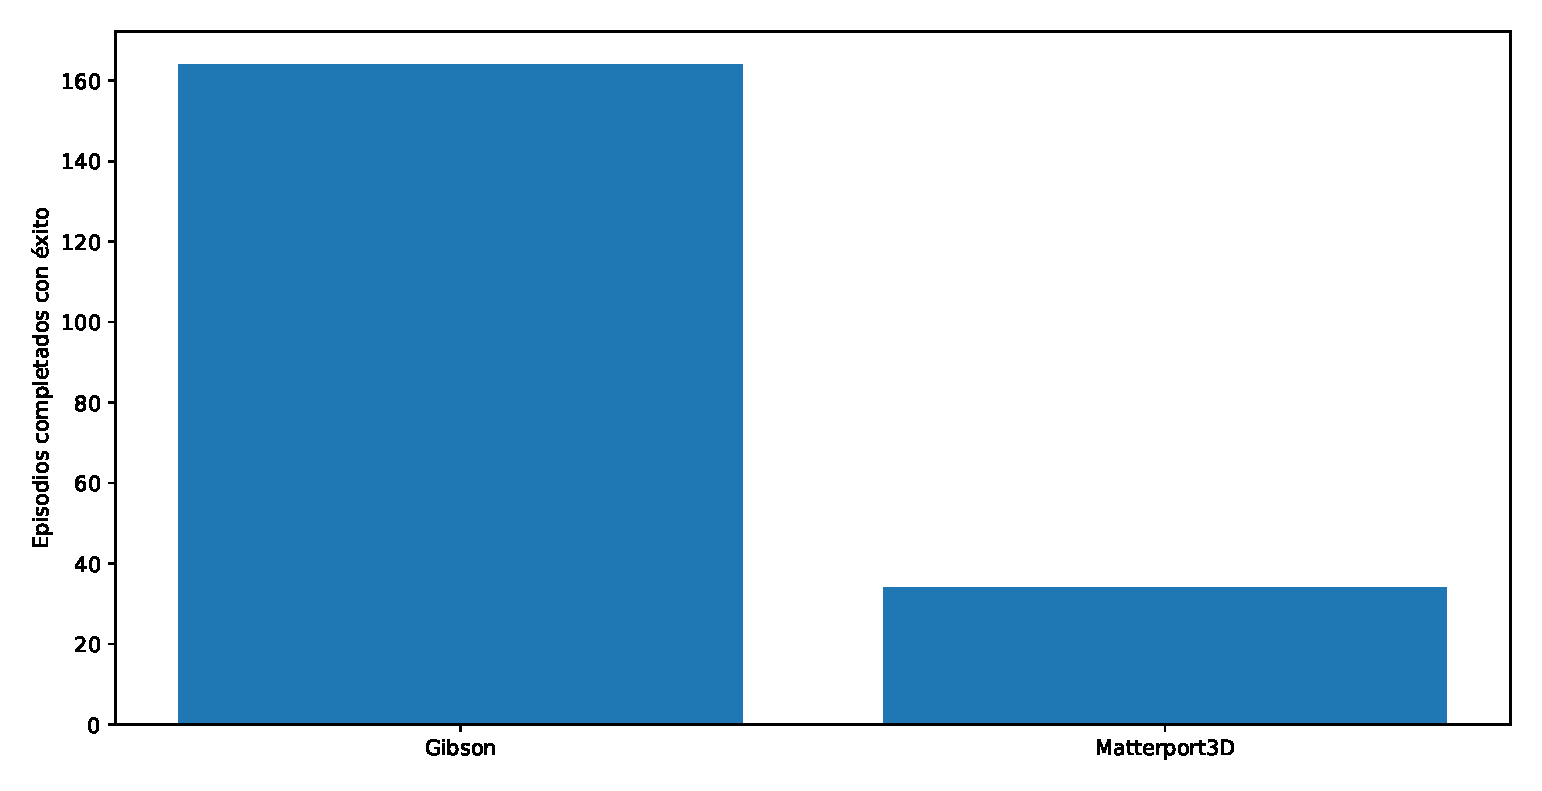
\includegraphics[width=0.9\textwidth]{imagenes/cap6/dataset/success.eps}
    \caption{Comparativa de conjuntos de datos - Episodios completados con éxito.}
    \label{fig:chap6-dataset-success}
\end{figure}

Por otra parte, si se compara el porcentaje de distancia recorrida por episodio, como se puede ver en la Figura \ref{fig:chap6-dataset-distance}, se puede ver un comportamiento más parecido entre ambos agentes. Los dos agentes empiezan a aumentar la distancia recorrida aproximadamente a partir de los 6000 episodios, creciendo hasta la franja de los 12000 episodios. Ahora bien, tras ese punto el rendimiento del agente de \textit{Matterport3D} baja notablemente, pasando a ser el agente de \textit{Gibson} ligeramente superior en esta métrica.

\begin{figure}[h]
    \centering
    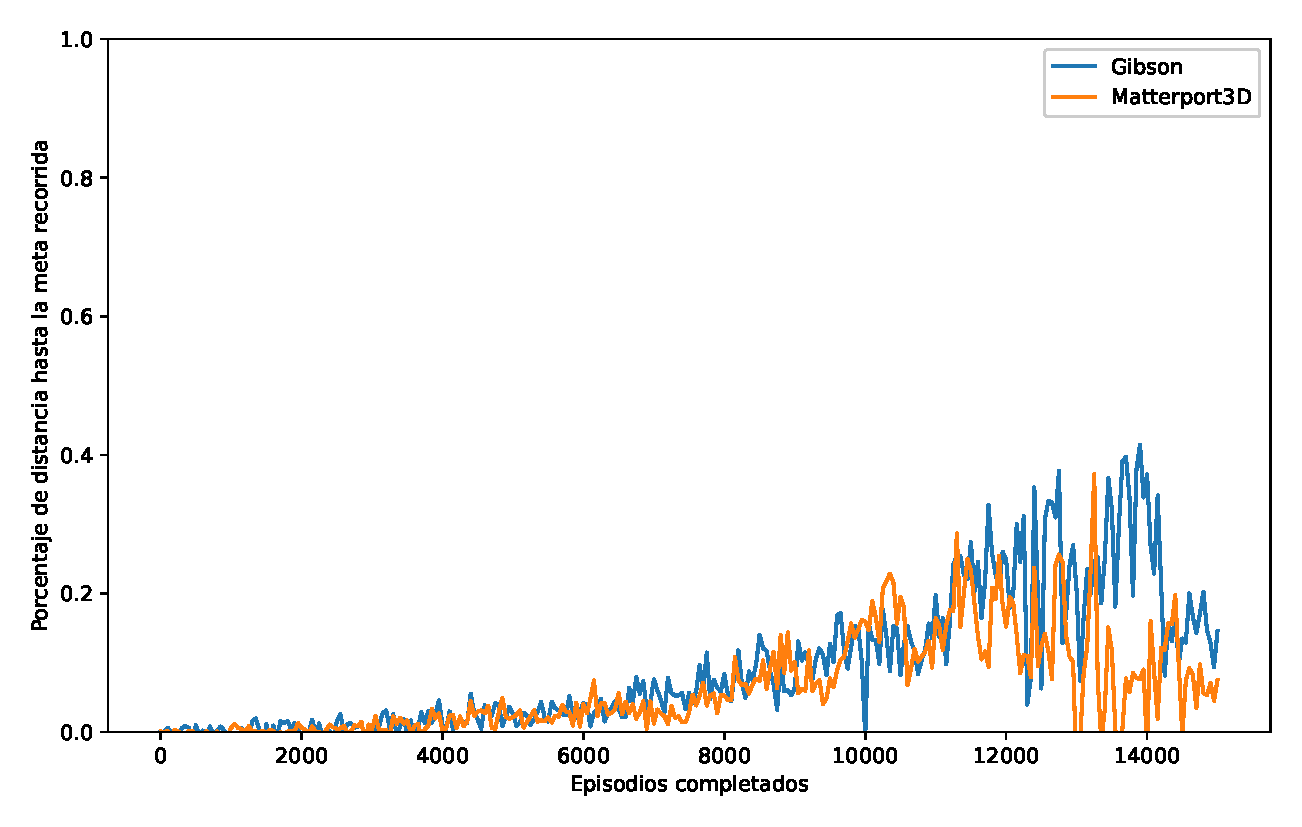
\includegraphics[width=0.9\textwidth]{imagenes/cap6/dataset/smoothed_distances.eps}
    \caption{Comparativa de conjuntos de datos - Distancia recorrida por episodio.}
    \label{fig:chap6-dataset-distance}
\end{figure}

Estas dos comparativas, junto a la experiencia previa de otros autores comparando ambos conjuntos de datos \cite{habitat19iccv} justifica nuestra elección de \textit{Gibson} como conjunto de datos para el entrenamiento, siendo éste el conjunto más simple y que mejores resultados ofrece.

\subsection{Agentes con \textit{Deep Q-Learning} estándar}

En la Figura \ref{fig:chap6-standard-success} se pueden ver las tasas de acierto de los cuatro agentes de esta propuesta. Se puede observar claramente que el agente usando \textbf{contornos} es el que más episodios ha sido capaz de completar (aproximadamente \textbf{160 episodios}), siendo dos veces superior al siguiente mejor agente, el agente usando \textbf{columnas} (con aproximadamente \textbf{80 episodios}). El agente usando \textbf{contornos con colisiones} obtiene resultados similares al agente de columnas, pero ligeramente inferiores (con aproximadamente \textbf{60} episodios). Finalmente, el agente de \textbf{columnas con colisiones} ofrece el peor resultado con cerca de \textbf{20} episodios, siendo notablemente peor al resto de agentes.

A primera vista se ve que la propuesta de recompensa original (usando contornos para identificar obstáculos) ofrece los mejores resultados al agente. Ahora bien, también se puede ver que el uso de detección de colisiones empeora el resultado considerablemente, en contra de su efecto en el trabajo original de Carlos Sampedro \textit{et al.} \cite{Sampedro2018}. Esto puede deberse a la mayor complejidad de los escenarios del conjunto de datos, donde las colisiones pueden resultar inevitables, provocando que el agente acabe en un bucle evitando colisiones sin lograr llegar a la meta en ningún momento.

\begin{figure}[H]
    \centering
    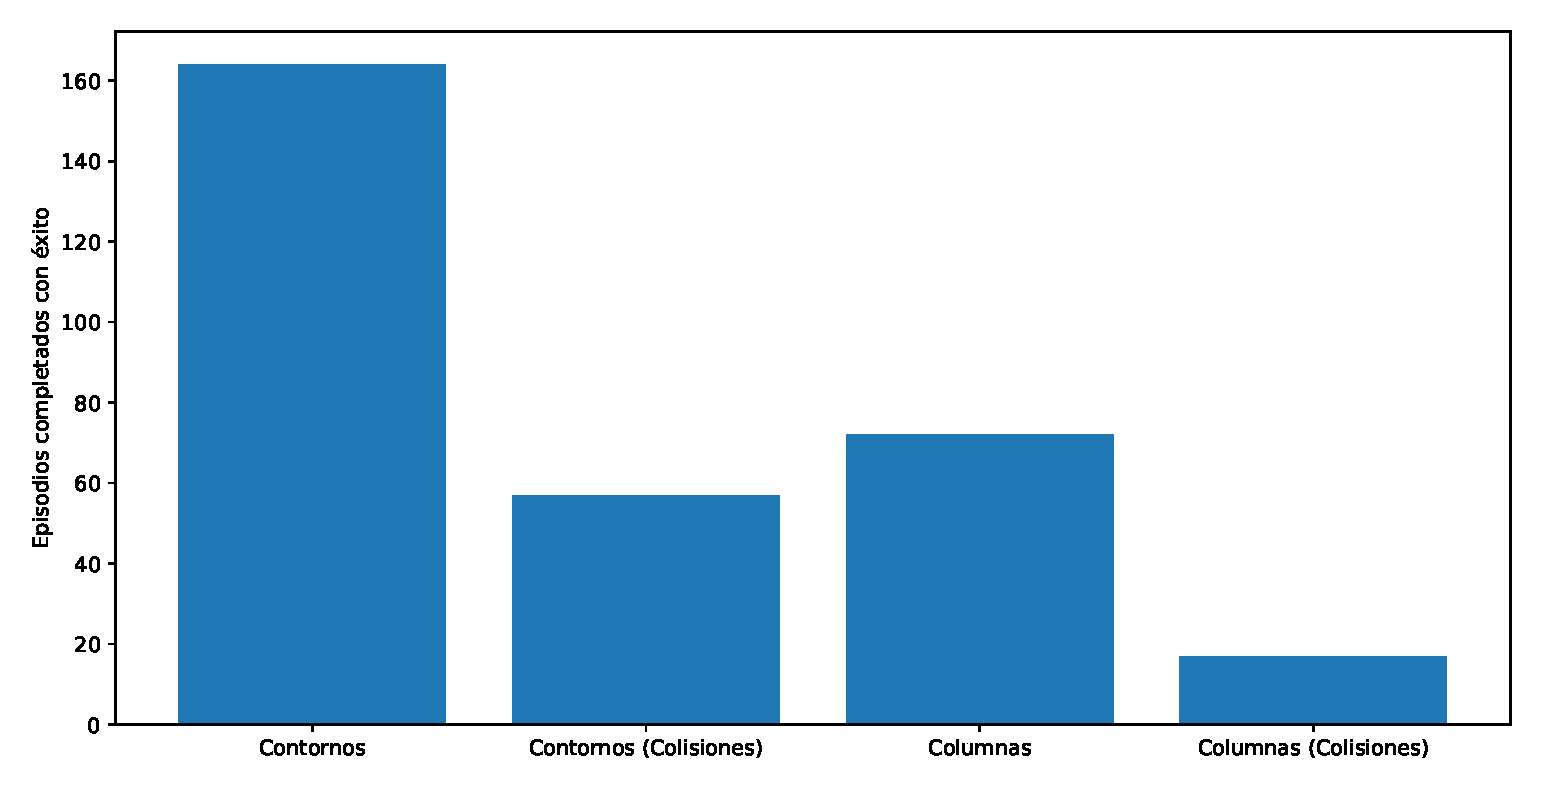
\includegraphics[width=0.9\textwidth]{imagenes/cap6/standard/success.eps}
    \caption{Agentes estándares - Episodios completados con éxito.}
    \label{fig:chap6-standard-success}
\end{figure}

Comparando los tiempos de entrenamiento - disponibles en la Figura \ref{fig:chap6-standard-time} - se pueden distinguir dos grupos claros: los agentes sin colisiones (usando \textbf{contornos} y \textbf{columnas}) siguen una curva prácticamente idéntica, necesitando aproximadamente \textbf{12} horas para sus entrenamientos, con un aumento rápido alrededor de los 12000 episodios que se empieza a normalizar hacia los 14000 episodios.

En cambio, los agentes con colisiones acaban su entrenamiento en menor tiempo, siendo más lento el agente de \textbf{columnas con colisiones} que su equivalente usando contornos. Como se verá a continuación, esto se debe al número de acciones realizadas.

\begin{figure}[H]
    \centering
    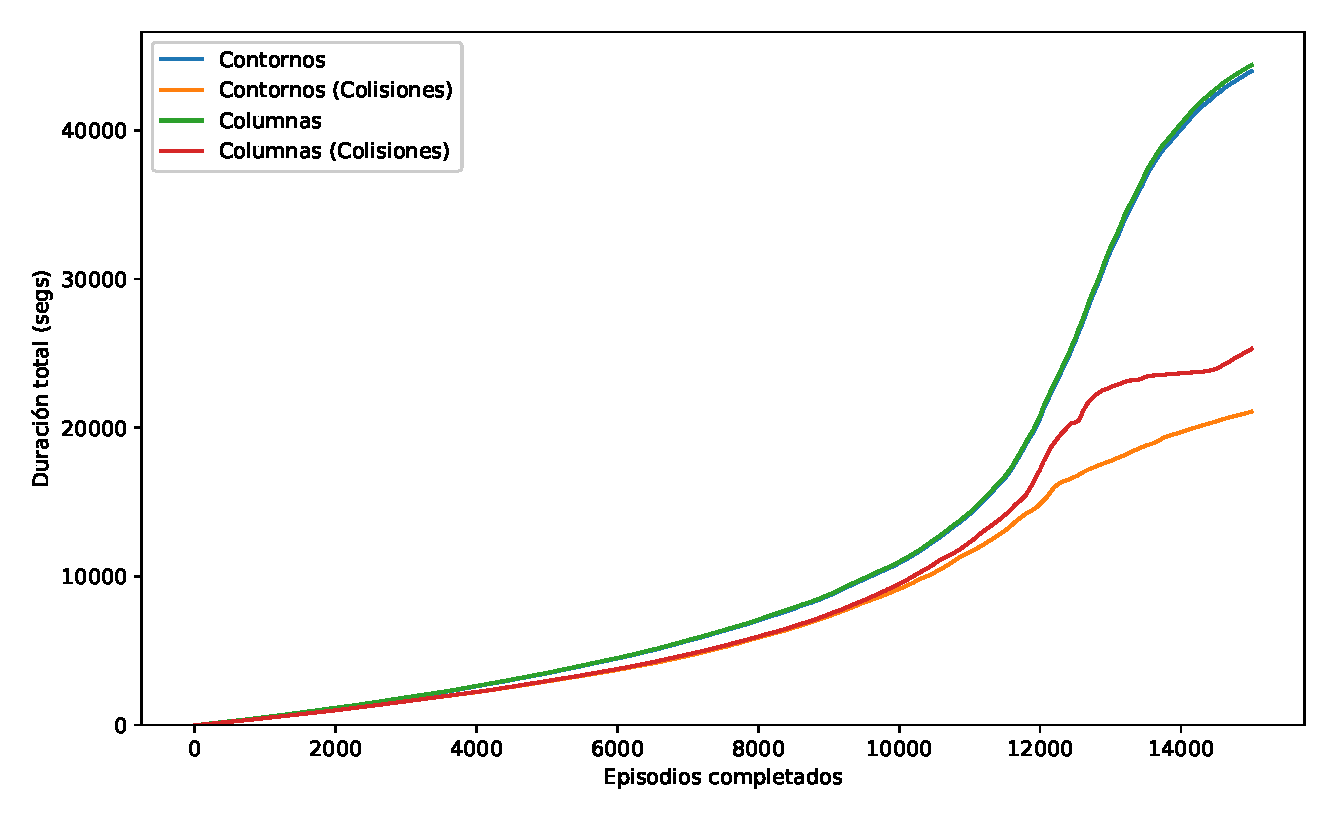
\includegraphics[width=0.9\textwidth]{imagenes/cap6/standard/cumulative_smoothed_times.eps}
    \caption{Agentes estándares - Tiempo total de entrenamiento.}
    \label{fig:chap6-standard-time}
\end{figure}

Estudiando las acciones realizadas por episodio - disponibles en la Figura \ref{fig:chap6-standard-actions} - se puede ver que el comportamiento de todos los agentes es similar hasta aproximadamente los 10000 episodios, aumentando paulatinamente el número de acciones realizadas conforme los agentes aprenden.

Ahora bien, a partir de ese punto se vuelven a separar los agentes en dos grupos, agentes con y sin colisiones. Los agentes sin colisiones de nuevo presentan gráficas prácticamente idénticas, teniendo un gran pico de acciones alrededor de los 12000 episodios, a partir del cual se vuelve a reducir rápidamente el número de acciones realizadas hasta los niveles previos al pico. Este pico corresponde aproximadamente con el punto en el que se alcanza el valor mínimo de epsilon, lo que puede indicar que la política del agente lo lleva a acabar los episodios rápidamente.

Los agentes con colisiones presentan un pico similar pero menos pronunciado, realizando el agente de \textbf{columnas con colisiones} un mayor número de acciones que su equivalente por contornos (si bien el número de acciones de ambos agentes es inestable). Ahora bien, tras su pico, el número de acciones realizadas por ambos agentes baja a niveles inferiores a los existentes antes del pico, aunque el agente de \textbf{columnas con colisiones} acaba recuperándose hasta llegar a un número similar al de los agentes sin colisiones.

\begin{figure}[H]
    \centering
    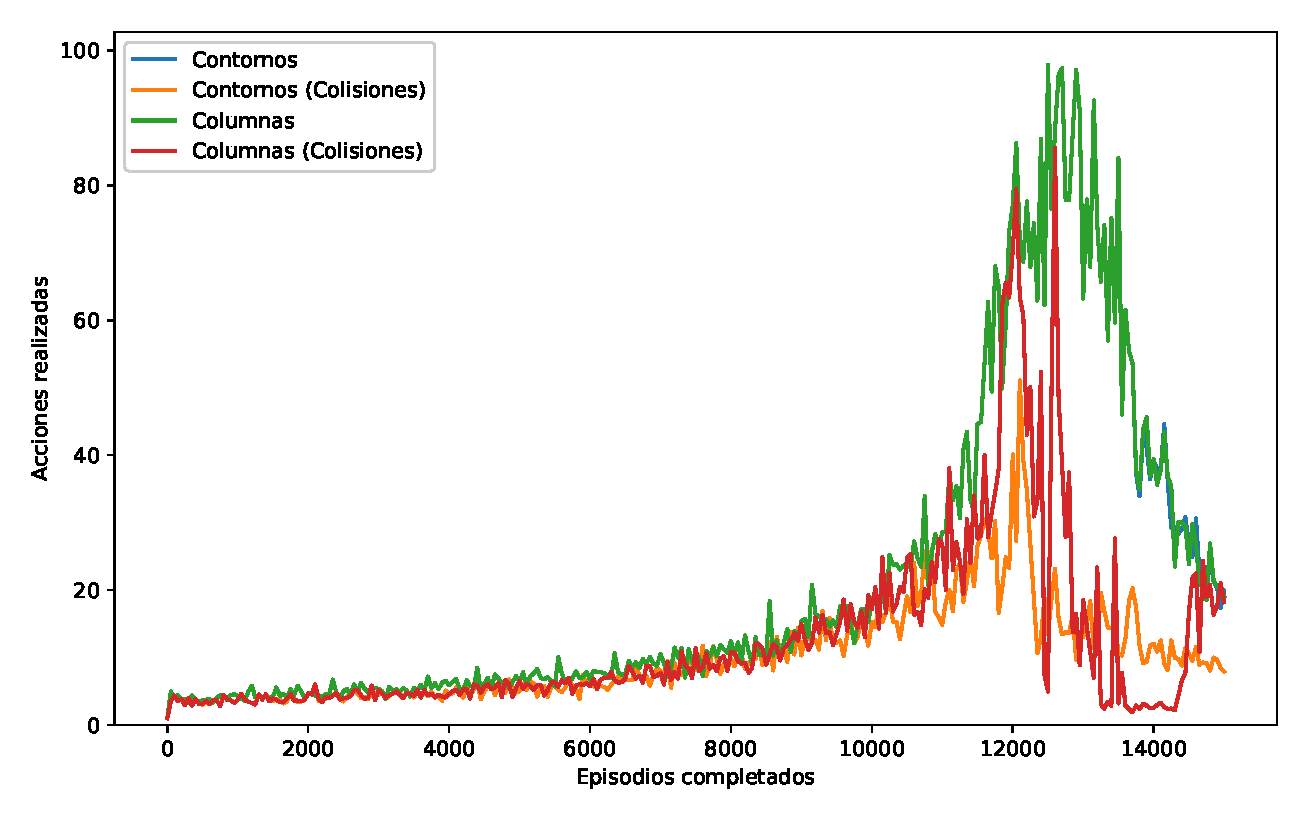
\includegraphics[width=0.8\textwidth]{imagenes/cap6/standard/smoothed_actions.eps}
    \caption{Agentes estándares - Acciones realizadas por episodio.}
    \label{fig:chap6-standard-actions}
\end{figure}

Comparando el porcentaje de distancia recorrida por episodio - disponible en la Figura \ref{fig:chap6-standard-distances} - es posible ver cómo los agentes empiezan a aumentar la distancia recorrida lentamente durante el entrenamiento, teniendo todos gráficas similares (si bien ruidosas) hasta los 10000 episodios.

Tras este punto, el rendimiento de los cuatro agentes empieza a mejorar pero de forma muy inestable, con picos superiores e inferiores en un rango amplio (entre el $0.0$ y el $0.4$). Tras aproximadamente 14000 episodios, la distancia recorrida por los agentes se acaba normalizando, ofreciendo los mejores resultados los agentes de \textbf{contornos sin y con colisiones}, recorriendo cerca del $20\%$ de la distancia de los episodios. El agente de \textbf{columnas sin colisiones} ofrece resultados peores pero que empiezan a mejorar al final, acabando cerca del $15\%$ de la distancia. Finalmente, el agente de \textbf{columnas con colisiones} empeora hasta ser incapaz de avanzar durante los episodios, quedándose alrededor del $0\%$ de la distancia recorrida (posiblemente incluso alejándose de la meta).

\begin{figure}[h]
    \centering
    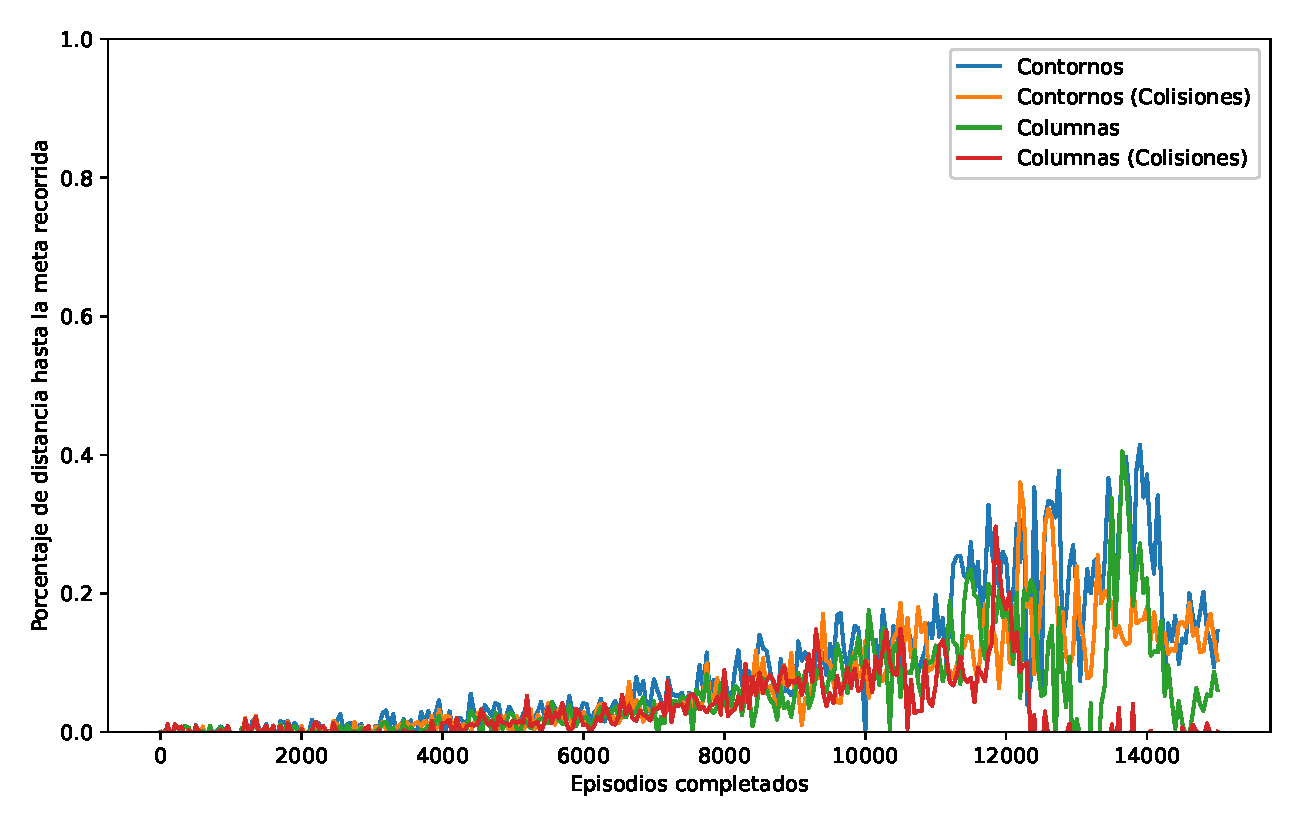
\includegraphics[width=0.9\textwidth]{imagenes/cap6/standard/smoothed_distances.eps}
    \caption{Agentes estándares - Distancia recorrida por episodio.}
    \label{fig:chap6-standard-distances}
\end{figure}

Finalmente, si se comparan las recompensas medias por episodio - disponibles en la Figura \ref{fig:chap6-standard-rewards} - se puede ver cómo la recompensa media mejora progresivamente hasta alcanzar los 12000 episodios aproximadamente (sin llegar a ser positiva en ningún momento). Este aumento se corresponde con el comportamiento observado del número de acciones y de la distancia recorrida.

A partir de ese punto, los agentes sin colisiones (\textbf{contornos} y \textbf{columnas}) tienen un valle (correspondiendo con el pico de acciones) a partir del cual empieza a descender la recompensa media por episodios. La recompensa media del agente de \textbf{contornos con colisiones} también presenta el valle y caída, si bien su recompensa media en general es inferior a la de los agentes sin colisiones.

El comportamiento más inesperado lo presenta el agente de \textbf{columnas con colisiones}, desplomándose su recompensa media en los 2500 últimos episodios, llegando a niveles inferiores a los valores iniciales (correspondiéndose con el bajo rendimiento del agente en la distancia). Aun así, estas recompensas se acaban recuperando, alcanzando el nivel aproximado del resto de agentes a los 15000 episodios.

\begin{figure}[H]
    \centering
    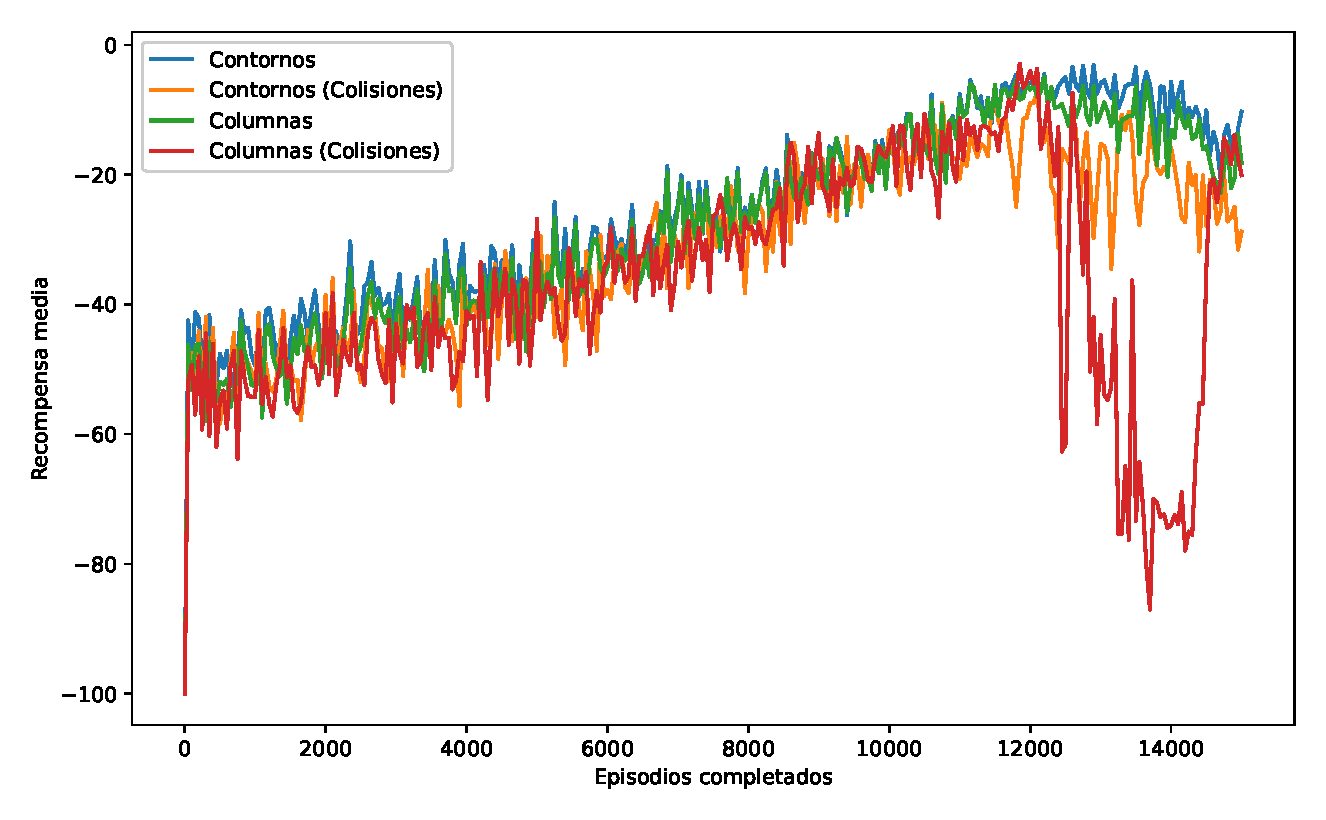
\includegraphics[width=0.9\textwidth]{imagenes/cap6/standard/smoothed_rewards.eps}
    \caption{Agentes estándares - Recompensa media por episodio.}
    \label{fig:chap6-standard-rewards}
\end{figure}

\subsection{Agentes con \textit{Deep Q-Learning} priorizado}

En la Figura \ref{fig:chap6-prioritized-success} se pueden ver las tasas de acierto de los cuatro agentes de esta propuesta. De nuevo, el mejor resultado lo ofrece el agente de \textbf{contornos sin colisiones}, completando aproximadamente \textbf{14} episodios con éxito. En comparativa, el resto de agentes ofrece resultados peores, siendo los siguientes mejores agentes (\textbf{contornos con colisiones} y \textbf{columnas sin colisiones}) aproximadamente cinco veces peores, con \textbf{3} episodios realizados con éxito. Finalmente el agente de \textbf{columnas con colisiones} ofrece los peores resultados, completando un único episodio con éxito.

\begin{figure}[h]
    \centering
    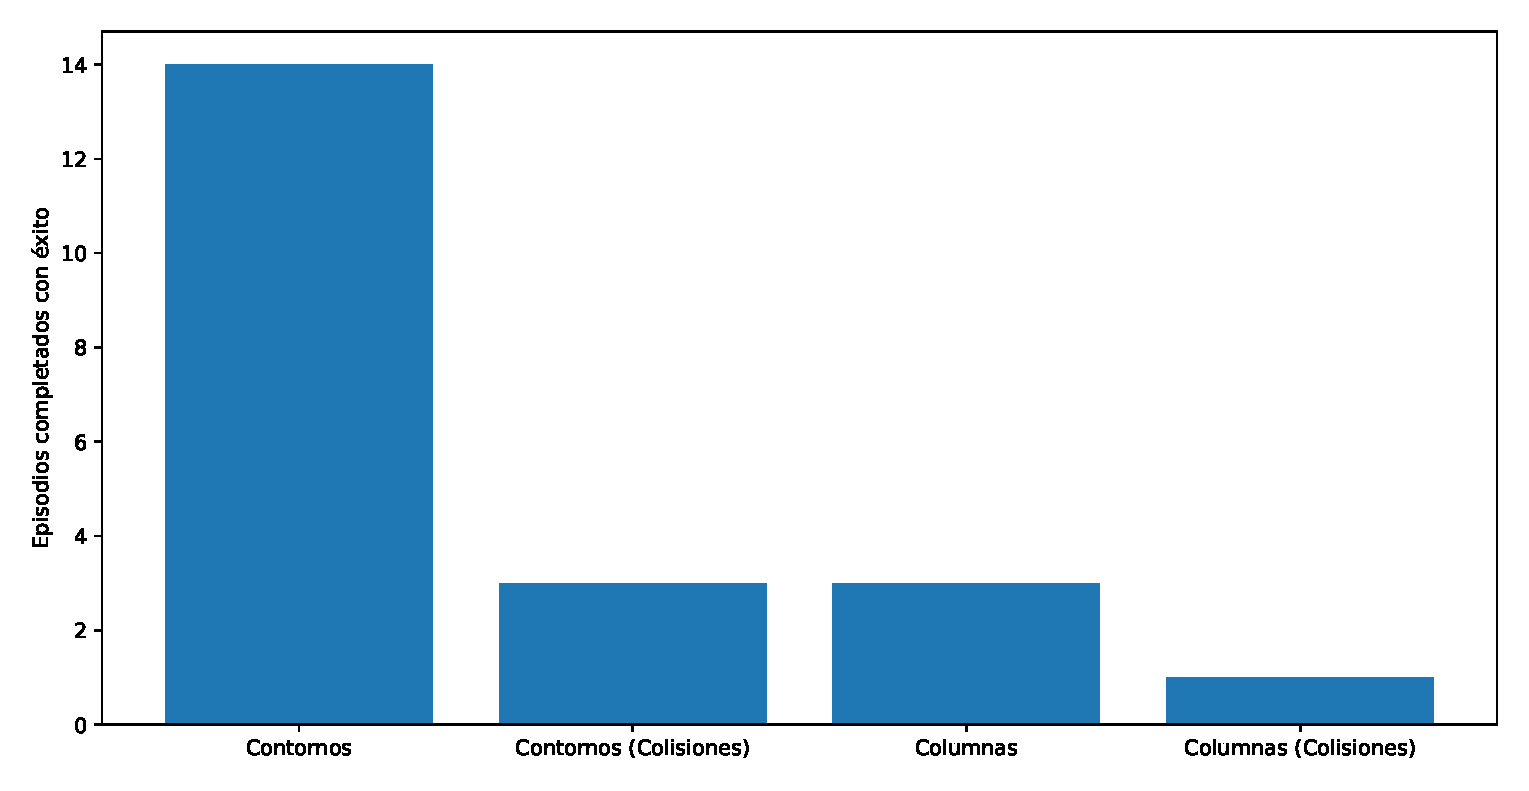
\includegraphics[width=0.9\textwidth]{imagenes/cap6/prioritized/success.eps}
    \caption{Agentes priorizados - Episodios completados con éxito.}
    \label{fig:chap6-prioritized-success}
\end{figure}

Los resultados son similares a los agentes de la primera propuesta, siendo la mejor opción la detección de obstáculos por contornos sin usar colisiones. Ahora bien, aunque puede parecer que los resultados son mucho peores a la primera aproximación (únicamente \textbf{14} episodios frente a los \textbf{160} del mejor agente), hay que tener en cuenta que los agentes priorizados han sido entrenados únicamente durante 3000 episodios, no pudiendo realizarse una comparación directa.

Si se comparan los tiempos de entrenamiento - disponibles en la Figura \ref{fig:chap6-prioritized-time} - se ve cómo los agentes sin colisiones (\textbf{contornos} y \textbf{columnas}) presentan un tiempo de entrenamiento prácticamente idéntico, siendo el más elevado de todos los agentes (tardando aproximadamente \textbf{6} horas en realizar el entrenamiento).

Ahora bien, en esta ocasión los agentes con colisiones se desmarcan entre ellos en la duración de su entrenamiento, siguiendo el agente de \textbf{columnas con colisiones} una trayectoria parecida a la de los agentes sin colisiones pero de menor altura, mientras que el tiempo de entrenamiento del agente de \textbf{contornos con colisiones} (el más rápido de todos) no tiene un crecimiento tan súbito como el resto de agentes.

\begin{figure}[h]
    \centering
    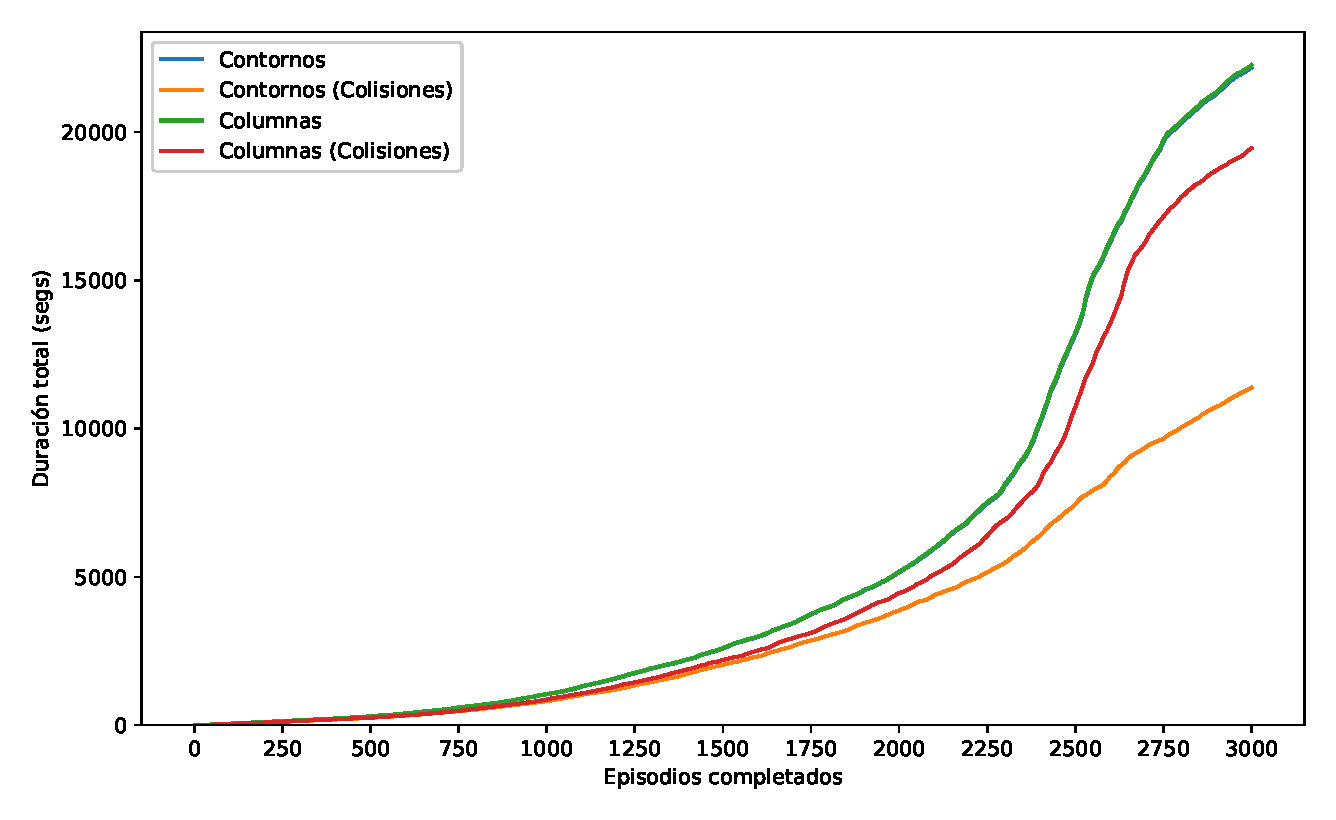
\includegraphics[width=0.9\textwidth]{imagenes/cap6/prioritized/cumulative_smoothed_times.eps}
    \caption{Agentes priorizados - Tiempo total de entrenamiento.}
    \label{fig:chap6-prioritized-time}
\end{figure}

Comparando las acciones realizadas por los agentes - como se puede ver en la Figura \ref{fig:chap6-prioritized-actions} - el comportamiento de los cuatro agentes es similar, teniendo un número de acciones (alrededor de \textbf{10} por episodio) constante hasta los 2000 episodios.

A partir de este punto, los agentes se empiezan a separar, siendo los agentes sin colisiones (\textbf{contornos} y \textbf{columnas}) los que más acciones realizan, con un pico de alrededor de \textbf{175} acciones por episodio a los 2500 episodios. Tras este pico el número de acciones vuelve a decrecer hasta estabilizarse alrededor de \textbf{25} acciones.

En los agentes con colisiones, el agente por \textbf{columnas} presenta un comportamiento similar, con un pico menor pero alcanzando unas acciones similares a los dos agentes anteriores. Ahora bien, el agente de \textbf{contornos con colisiones} no presenta un pico, manteniéndose el número de acciones alrededor de \textbf{25} todos los episodios hasta el final del entrenamiento.

\begin{figure}[h]
    \centering
    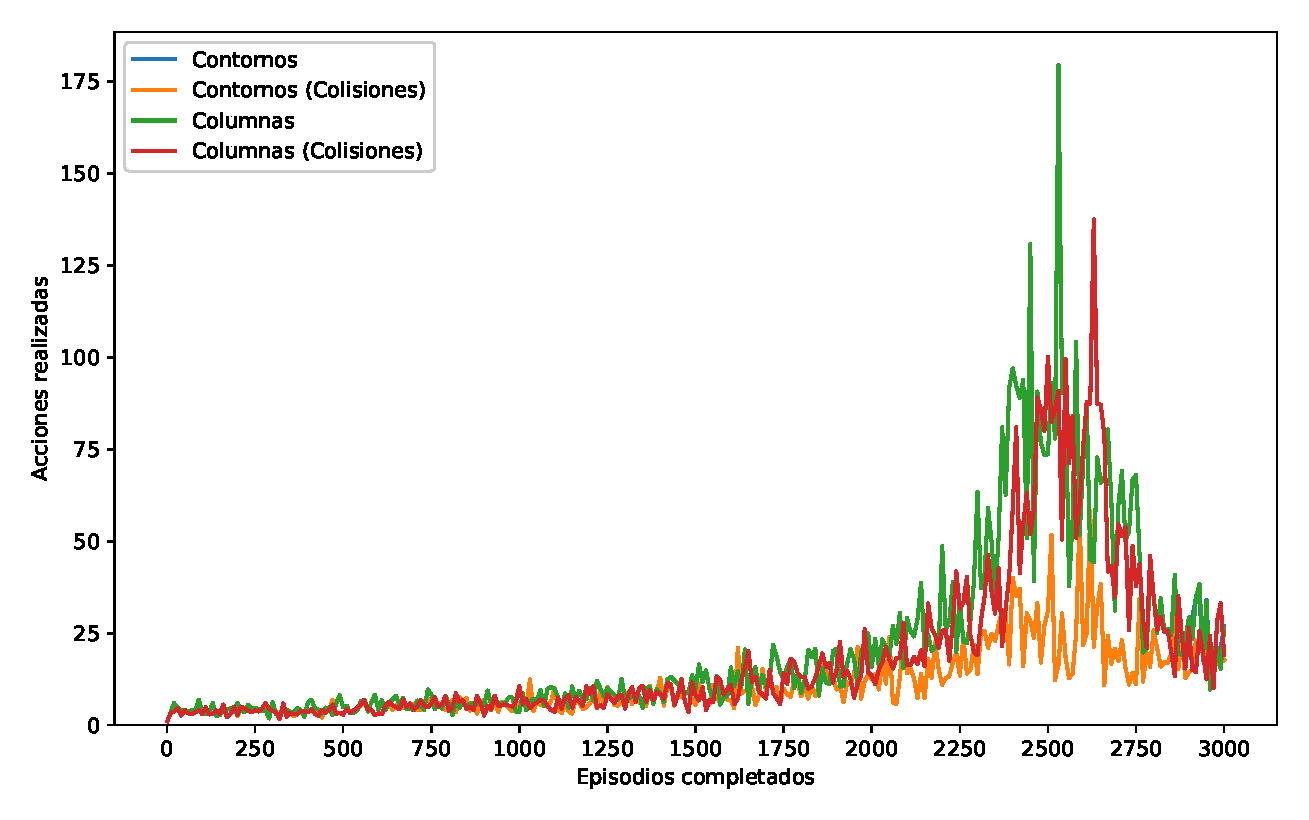
\includegraphics[width=0.9\textwidth]{imagenes/cap6/prioritized/smoothed_actions.eps}
    \caption{Agentes priorizados - Acciones realizadas por episodio.}
    \label{fig:chap6-prioritized-actions}
\end{figure}

Estudiando el porcentaje de distancia recorrida por cada agente - disponible en la Figura \ref{fig:chap6-prioritized-distances} - se puede ver como todos los agentes presentan un comportamiento similar durante todo el entrenamiento: la distancia recorrida media aumenta lentamente durante todo el entrenamiento, siendo esta distancia inestable en el rango de los 2000 a los 2750 episodios. Tras esto, el porcentaje medio de distancia recorrida se normaliza alrededor del $10\%$ de la distancia total.

\begin{figure}[H]
    \centering
    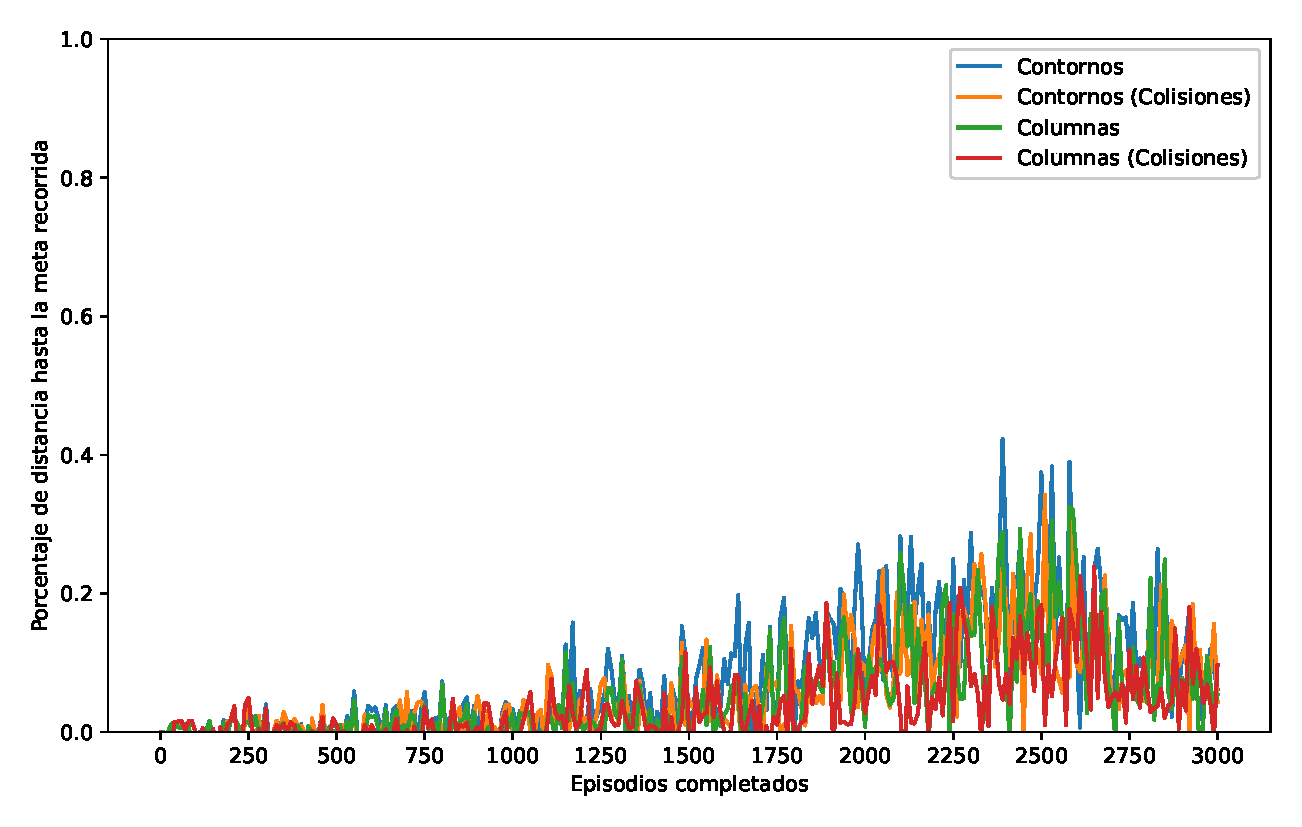
\includegraphics[width=0.9\textwidth]{imagenes/cap6/prioritized/smoothed_distances.eps}
    \caption{Agentes priorizados - Distancia recorrida por episodio.}
    \label{fig:chap6-prioritized-distances}
\end{figure}

Las únicas diferencia en el comportamiento de los agentes son que el agente de \textbf{contornos sin colisiones} presenta picos mayores durante el entrenamiento, y que el agente de \textbf{columnas con colisiones} recorre una distancia ligeramente menor de media durante el entrenamiento.

Finalmente, comparando la recompensa media por episodio - como se puede ver en la Figura \ref{fig:chap6-prioritized-rewards} - se ve que, de forma parecida a la distancia y a las acciones, los agentes presentan un comportamiento muy parecido durante todo el entrenamiento, aumentando la recompensa media lentamente hasta aproximadamente los 2500 episodios, punto tras el cual se reduce levemente la recompensa media.

Ahora bien, al contrario de la distancia o las acciones, cuyos valores se vuelven más ruidosos y oscilantes conforme aumenta el entrenamiento, la recompensa media se vuelve más consistente, alcanzando un valle alrededor de los 2500 episodios. De igual manera, el descenso tras este valle es apenas pronunciado, alcanzando una recompensa media de $-20$ durante el final del entrenamiento de manera consistente.

\begin{figure}[h]
    \centering
    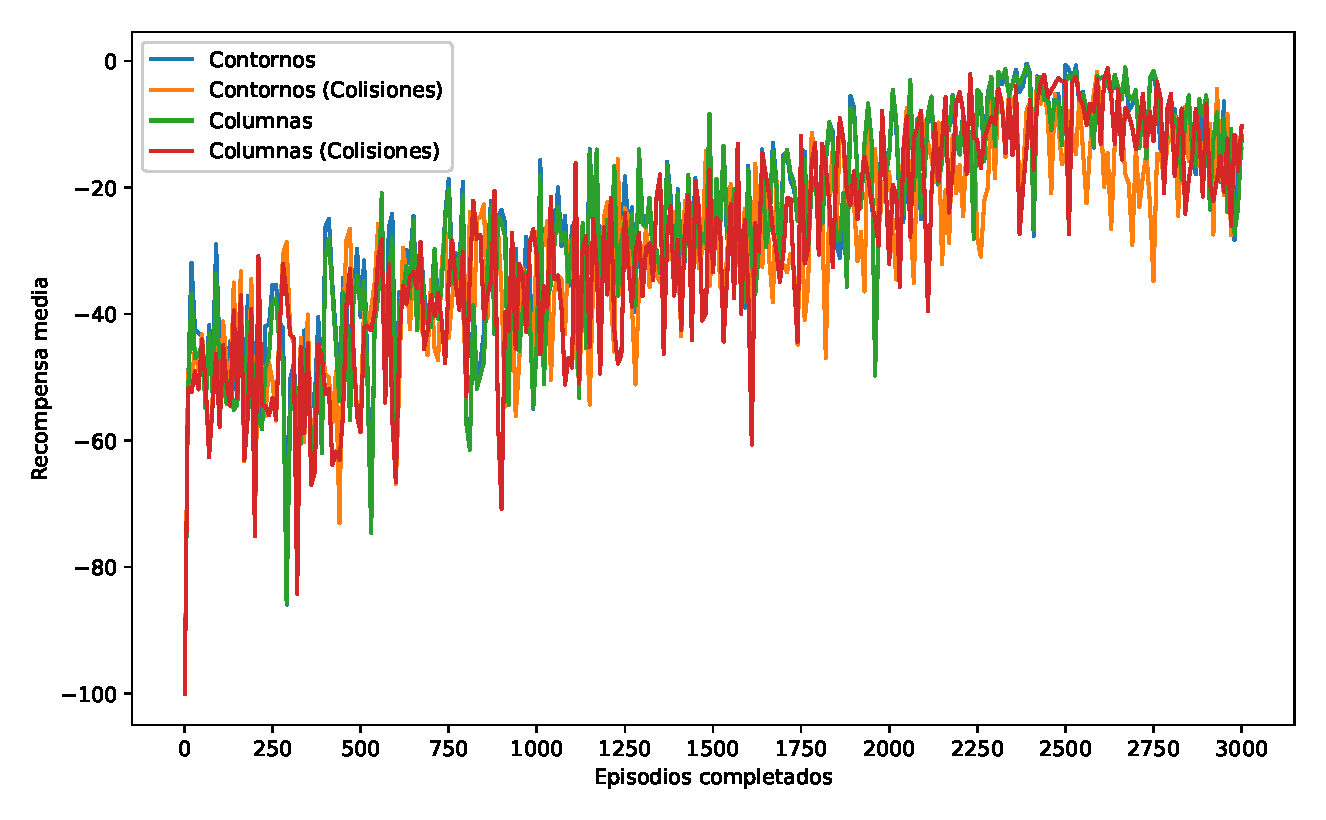
\includegraphics[width=0.9\textwidth]{imagenes/cap6/prioritized/smoothed_rewards.eps}
    \caption{Agentes priorizados - Recompensa media por episodio.}
    \label{fig:chap6-prioritized-rewards}
\end{figure}

\section{Comparativa y análisis de los resultados}

En esta sección se comparan los resultados de la experimentación realizada, tanto durante el entrenamiento (comparando a los mejores agentes de los dos grupos anteriores) como durante la evaluación, usando las métricas mencionadas previamente.

Finalmente, se realiza un análisis de todos los resultados obtenidos, extrayendo unas conclusiones al respecto.

\subsection{Comparativa durante el entrenamiento}

Para la comparativa, se han elegido los mejores dos agentes de cada una de las aproximaciones, siendo los agentes escogidos:
\begin{itemize}
	\item Agente de \textbf{contornos} sin colisiones (Estándar)
	\item Agente de \textbf{columnas} sin colisiones (Estándar)
	\item Agente de \textbf{contornos} sin colisiones (Priorizado)
	\item Agente de \textbf{columnas} sin colisiones (Priorizado)
\end{itemize}

Como se puede ver, los agentes con \textbf{colisiones} han sido descartados, al ofrecer peores rendimientos en general. Esto puede deberse a la complejidad de los escenarios (interiores de domicilios amueblados) donde las penalizaciones de las restricciones pueden resultar demasiado limitantes durante el entrenamiento.

Además, no es posible comparar directamente los dos grupos de agentes, al haber sido entrenados durante un número distinto de episodios (15000 episodios para los agentes estándares y 3000 episodios para los agentes priorizados). Por esto, para realizar una comparación más honesta, se ha optado por comparar el rendimiento de ambas familias de agentes durante los primeros 3000 episodios de entrenamiento.

Comparando la tasa de acierto de los agentes - como se puede ver en la Figura \ref{fig:chap6-comparison-success} - los agentes priorizados son claramente capaces de aprender en menos episodios una política capaz de finalizar episodios. El agente de \textbf{contornos priorizado} es el mejor agente en este caso, siendo capaz de acabar \textbf{14} episodios exitosamente, frente a los \textbf{3} episodios del agente de \textbf{columnas priorizado}. En cambio, los agentes \textbf{estándares} no acaban ningún episodio con éxito.

Ésto se corresponde con lo esperado al comparar ambas propuestas: \textit{Deep Q-Learning} con \textit{Prioritized Experience Replay} aprende muestreando memorias con más error (y por tanto, más importantes) del \textit{Replay Memory}, lo que acelera su proceso de entrenamiento. Esto se traduce en políticas más exitosas en un menor número de episodios.

\begin{figure}[h]
    \centering
    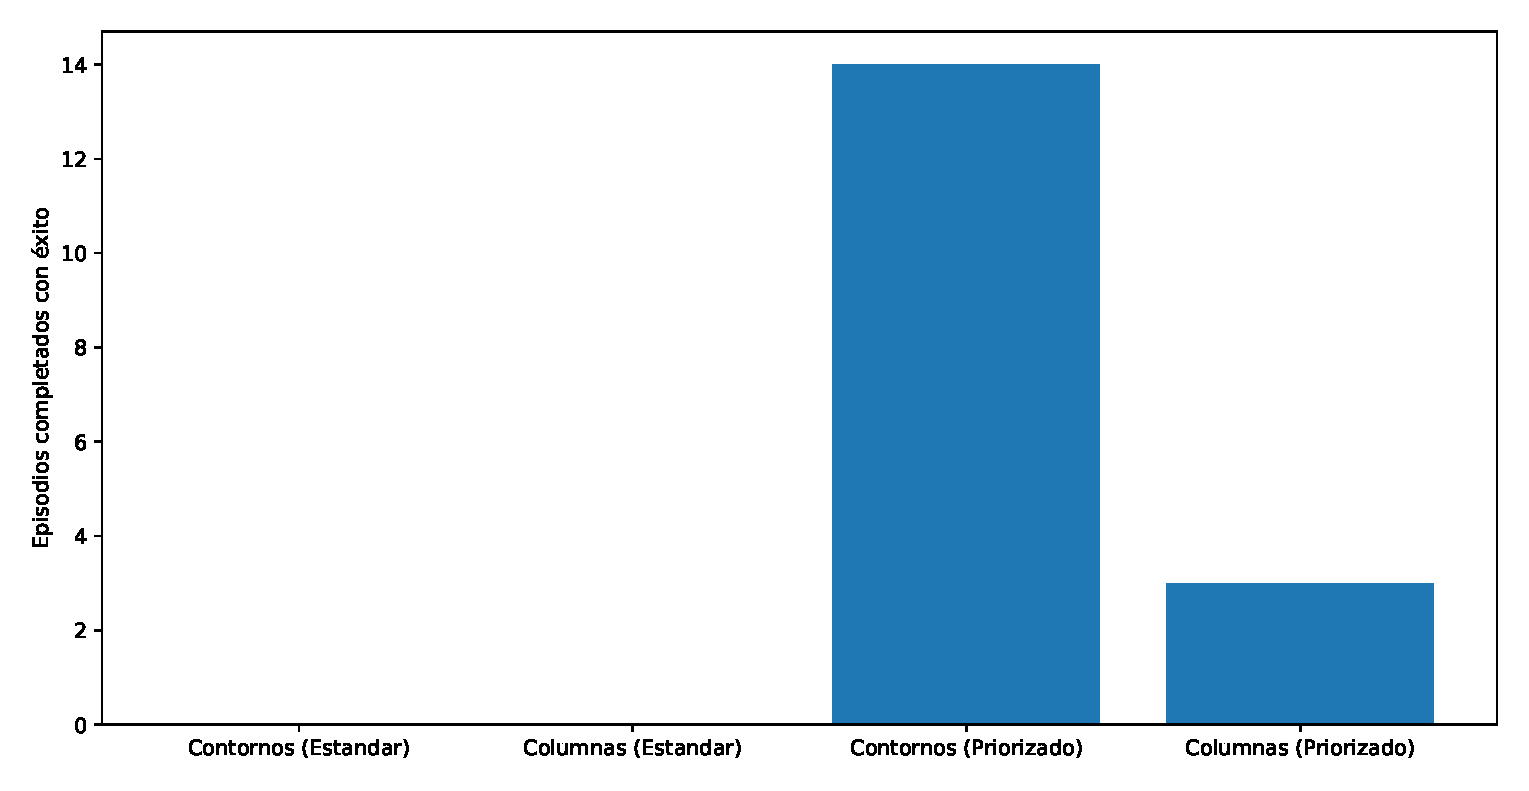
\includegraphics[width=0.8\textwidth]{imagenes/cap6/comparison/success.eps}
    \caption{Comparativa de agentes durante el entrenamiento - Episodios completados con éxito.}
    \label{fig:chap6-comparison-success}
\end{figure}

Respecto al tiempo total de entrenamiento - representado en la Figura \ref{fig:chap6-comparison-time} - se ve una diferencia clara entre las dos familias de agentes. Los agentes priorizados (\textbf{contornos priorizado} y \textbf{columnas priorizado}) necesitan un tiempo de entrenamiento mucho mayor al de los agentes estándares, tardando aproximadamente \textbf{22500} segundos (unas \textbf{6} horas) en simular 3000 episodios, frente a los \textbf{2500} segundos (aproximadamente \textbf{una} hora) de los agentes estándares.

Este resultado también es coherente con las técnicas utilizadas. Si bien el aprendizaje de \textit{Deep Q-Learning} con \textit{Prioritized Experience Replay} es más rápido (se necesitan menos episodios para que el agente aprenda una política), este aprendizaje también tiene un coste computacional mayor (al tener que realizar varios cálculos de distribuciones de probabilidad para cada muestreo), traduciéndose ésto en un mayor tiempo de entrenamiento.

\begin{figure}[h]
    \centering
    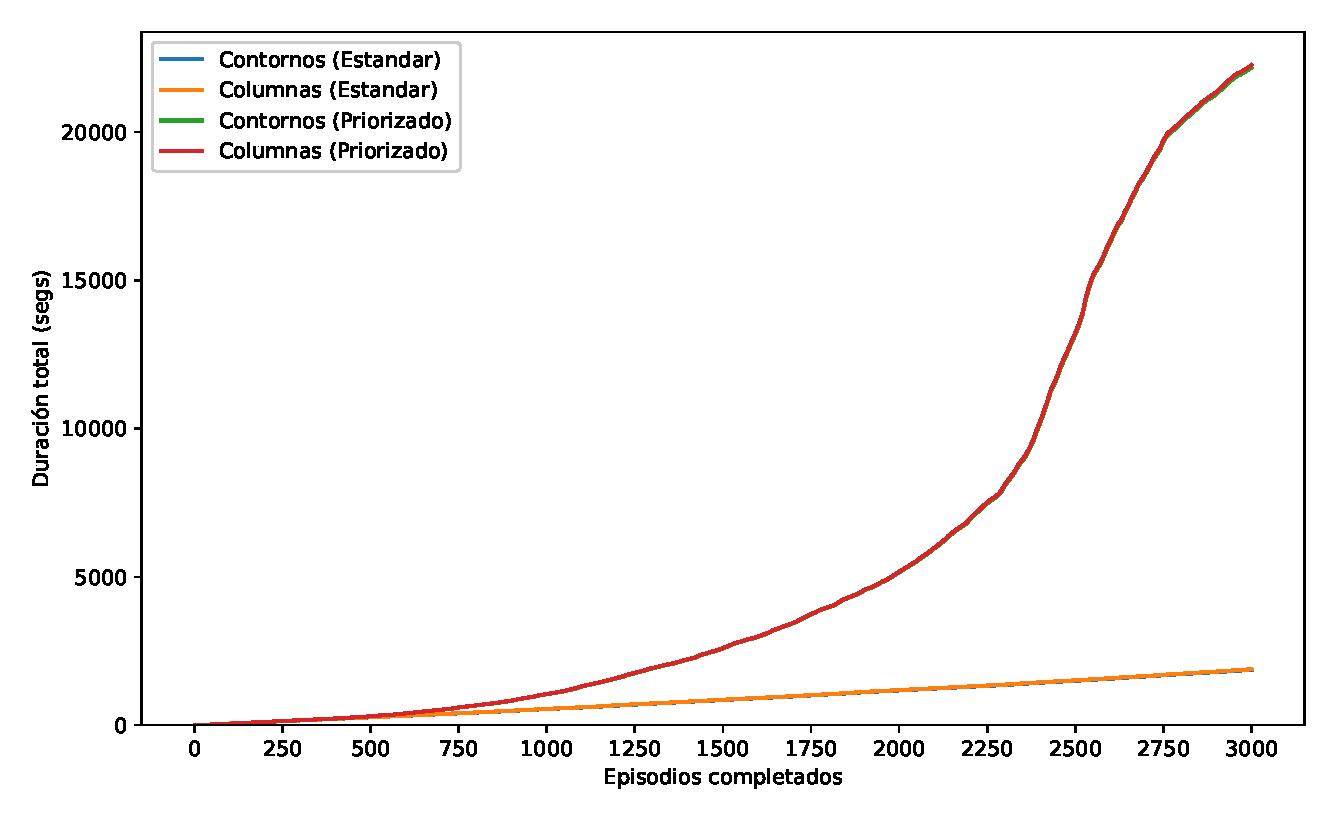
\includegraphics[width=0.8\textwidth]{imagenes/cap6/comparison/cumulative_smoothed_times.eps}
    \caption{Comparativa de agentes durante el entrenamiento - Tiempo total de entrenamiento.}
    \label{fig:chap6-comparison-time}
\end{figure}

Observando las acciones realizadas durante el entrenamiento - representadas en la Figura \ref{fig:chap6-comparison-actions} - se ve que los agentes priorizados siguen la forma que se ha dado hasta ahora: un crecimiento paulatino hasta que se acerca el final del entrenamiento, tras el cual alcanzan un pico de acciones y vuelve a estabilizarse el número de acciones promedio. 

En cambio, los agentes estándares no han sido capaces de aumentar el número de acciones realizadas en 3000 episodios, manteniéndose constante alrededor de las \textbf{5} acciones. Esto puede deberse a la falta de aprendizaje de los agentes estándares, provocando que realice acciones aleatorias en la práctica, frente a la política entrenada de los agente priorizados.

\begin{figure}[h]
    \centering
    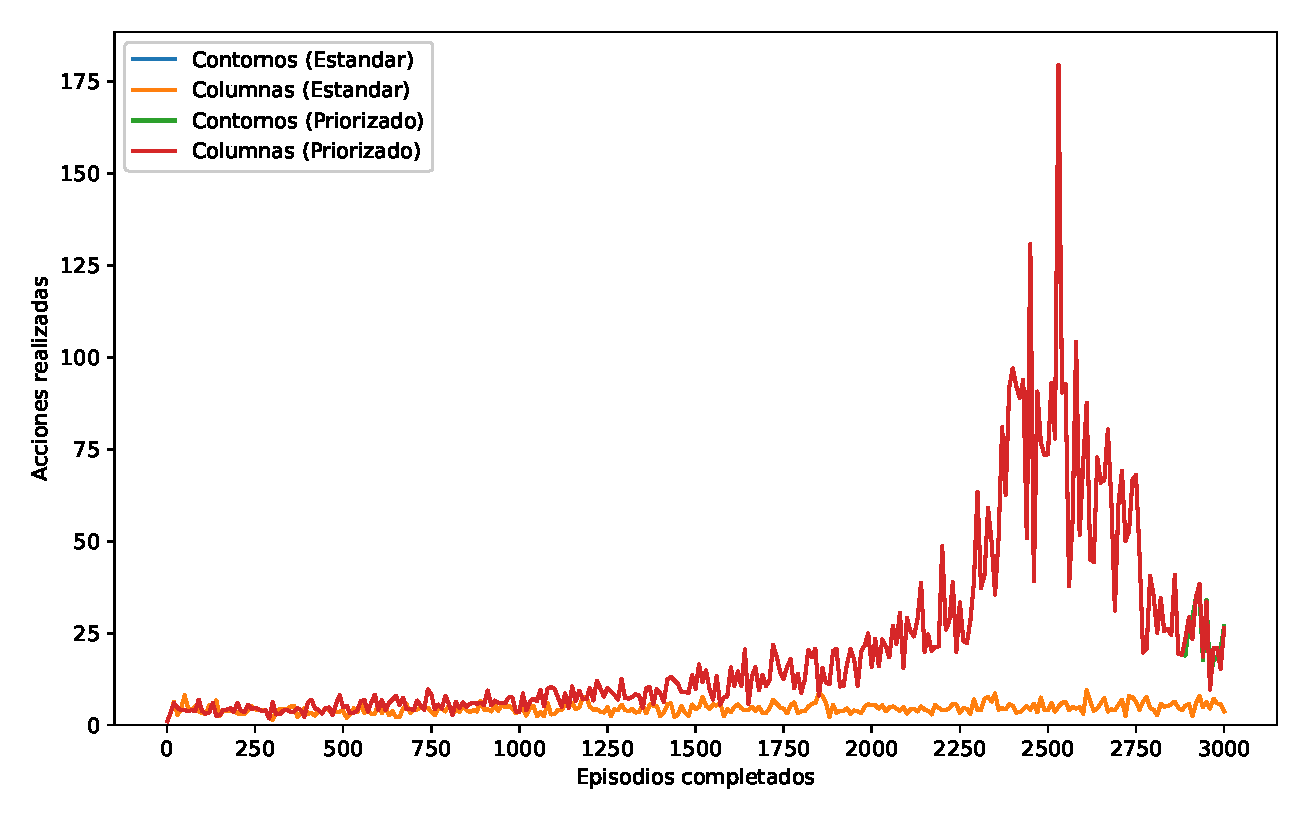
\includegraphics[width=0.8\textwidth]{imagenes/cap6/comparison/smoothed_actions.eps}
    \caption{Comparativa de agentes durante el entrenamiento - Acciones realizadas por episodio.}
    \label{fig:chap6-comparison-actions}
\end{figure}

Comparando la distancia recorrida por los agentes - disponible en la Figura \ref{fig:chap6-comparison-distances} - se vuelve a ver una separación entre el rendimiento de ambos tipos de agentes. Los agentes priorizados mejoran su rendimiento más rápidamente, empezando a recorrer distancias mayores a partir de los 1000 episodios y mejorando hasta un pico a los 2500 episodios (si bien su rendimiento es inestable, con picos notables). Tras este pico, se vuelve a estabilizar el rendimiento del agente, recorriendo de media alrededor del $15\%$ de la distancia. Ahora bien, el agente de \textbf{contornos priorizado} recorre una distancia ligeramente superior, si bien se puede afirmar que son equivalentes en la práctica.

\newpage

Frente a esto, los agentes estándares recorren en promedio una distancia mucho menor, mejorando ligeramente su resultado a partir de los 2000 episodios pero sin superar valores de aproximadamente el $5\%$. De nuevo, esto demuestra la velocidad de aprendizaje de \textit{Prioritized Experience Replay} (siendo capaz de recorrer una distancia mayor en menor número de episodios que los agentes estándares).

\begin{figure}[h!]
    \centering
    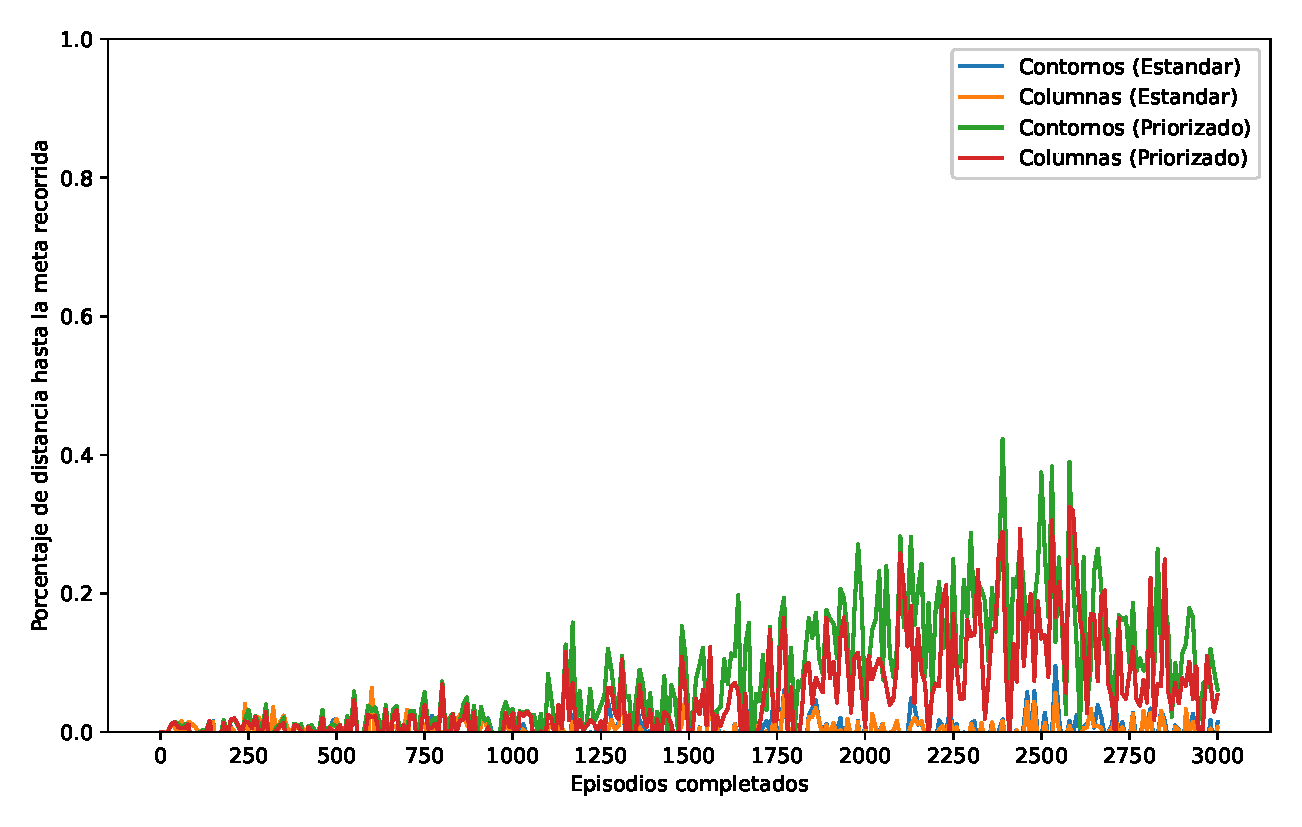
\includegraphics[width=0.8\textwidth]{imagenes/cap6/comparison/smoothed_distances.eps}
    \caption{Comparativa de agentes durante el entrenamiento - Distancia recorrida por episodio.}
    \label{fig:chap6-comparison-distances}
\end{figure}

Finalmente, comparando las recompensa media obtenida por los agentes - como se puede observar en la Figura \ref{fig:chap6-comparison-rewards} - se observa como los agentes priorizados presentan un comportamiento muy parecido, mejorando su recompensa media (sin llegar a valores positivos), alcanzando un techo alrededor de los 2500 episodios. Tras este techo, las recompensas acaban disminuyendo ligeramente y normalizándose por encima de $-20$.

Como comparación, los agentes estándares tienen una recompensa media con un crecimiento mucho más lento y estable, manteniéndose la recompensa media alrededor de $-40$.

De nuevo, el comportamiento de las recompensas se corresponde con lo visto hasta el momento. Los agentes priorizados realizan un mayor número de acciones (lo que acerca la recompensa media hacia $0$), y además realizan un aprendizaje más rápido (llevando a acciones con recompensas mayores y, por tanto, una recompensa promedio más elevada).

\begin{figure}[h]
    \centering
    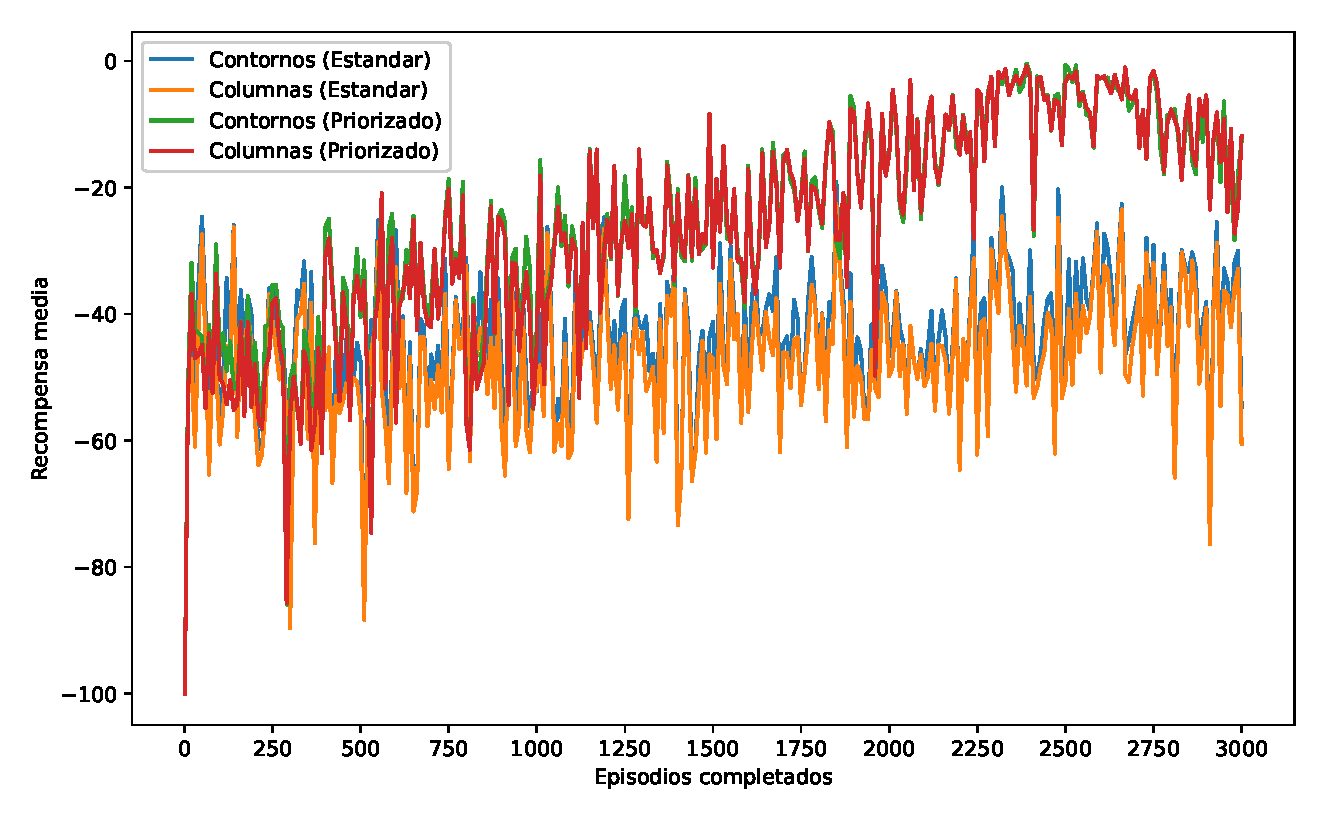
\includegraphics[width=0.8\textwidth]{imagenes/cap6/comparison/smoothed_rewards.eps}
    \caption{Comparativa de agentes durante el entrenamiento - Recompensa media por episodio.}
    \label{fig:chap6-comparison-rewards}
\end{figure}

\subsection{Comparativa durante la evaluación}

De cara a poder estimar el rendimiento real de los agentes al enfrentarse a problemas desconocidos (problemas nuevos en entornos no incluidos en el conjunto de entrenamiento) se procede a comparar su rendimiento ante un conjunto de evaluación separado del conjunto de datos usado durante el entrenamiento.

Se evaluará el rendimiento de todos los agentes durante un total de \textbf{250 episodios}. Además de los agentes entrenados (cuyo rendimiento se ha descrito en las secciones previas), se incluye en la comparativa una serie de agentes ofrecidos por defecto por \textit{Habitat}:

\begin{itemize}
	\item \textbf{baselines:} Agentes simples usados como base. Se espera que el agente propuesto presente un rendimiento superior a los agentes de \textit{baseline}, siendo éstos:
	\begin{itemize}
	\item \textit{random:} Un agente puramente aleatorio, el agente realiza una acción aleatoria en cada paso.
	\item \textit{random{\_}forward:} Una variante del agente \textit{random} con sesgo hacia el movimiento hacia alante. El agente avanza el $80\%$ de las acciones, teniendo un $20\%$ de posibilidades de rotar.
	\item \textit{goal{\_}follower:} Un agente heurístico simple, que rota hasta estar enfocado hacia la meta. Tras ésto, el agente procede a moverse hacia delante sin tener en cuenta ningún obstáculo.
	\end{itemize}
	
	Es importante destacar que los agentes aleatorios ofrecidos por \textit{Habitat} no son puramente aleatorios, sino que utilizan información adicional. Concretamente, los agentes aleatorios no pueden elegir al azar la acción \textbf{STOP} (para detener el episodio). En su lugar, conocen la distancia a la meta, utilizando automáticamente la acción si el agente alcanza la meta.
	
	\item \textbf{ppo:} Un agente utilizando el algoritmo de \textit{Proximal Policy Optimization} con un sistema de recompensas básico ofrecido por \textit{Habitat}. Este agente se utiliza como \textbf{objetivo}, siendo los resultados de este agente los resultados que se busca alcanzar.
	
\end{itemize}

Los resultados de esta evaluación se pueden observar en el Cuadro \ref{tab:results}. El agente con los mejores resultados de cada grupo se encuentra indicado en negrita.

\begin{table}[h]
\centering
\resizebox{\textwidth}{!}{%
\begin{tabular}{@{}ccrrrrr@{}}
\cmidrule(l){2-7}
\multicolumn{1}{l}{}                                                           & \textbf{Agente}                                                            & \multicolumn{1}{c}{\textbf{\begin{tabular}[c]{@{}c@{}}Distancia a\\ la meta (m)\end{tabular}}} & \multicolumn{1}{l}{\textbf{\begin{tabular}[c]{@{}l@{}}Tasa de\\ éxito\end{tabular}}} & \multicolumn{1}{l}{\textbf{SPL}} & \multicolumn{1}{l}{\textbf{SPL suavizado}} & \multicolumn{1}{c}{\textbf{Colisiones}} \\ \midrule
\multirow{3}{*}{Baselines}                                                     & \begin{tabular}[c]{@{}c@{}}Aleatorio\\ (Habitat)\end{tabular}              & 6.5227                                                                                         & 0.076                                                                                & 0.0512                           & 0.0845                                     & 139.228                                 \\ \cmidrule(l){2-7} 
                                                                               & \begin{tabular}[c]{@{}c@{}}Aleatorio\\ (Forward)\end{tabular}              & 6.3152                                                                                         & 0.032                                                                                & 0.0264                           & 0.0638                                     & 379.344                                 \\ \cmidrule(l){2-7} 
                                                                               & \textbf{\begin{tabular}[c]{@{}c@{}}Goal\\ Follower\end{tabular}}           & \textbf{3.2310}                                                                                & \textbf{0.352}                                                                       & \textbf{0.3502}                  & \textbf{0.3886}                            & \textbf{318.552}                        \\ \midrule
\multirow{4}{*}{\begin{tabular}[c]{@{}c@{}}Agentes\\ estándares\end{tabular}}  & Contornos                                                                  & 5.7175                                                                                         & 0.0                                                                                  & 0.0                              & 0.1179                                     & 364.944                                 \\ \cmidrule(l){2-7} 
                                                                               & Columnas                                                                   & 5.3395                                                                                         & 0.0                                                                                  & 0.0                              & 0.1096                                     & 224.292                                 \\ \cmidrule(l){2-7} 
                                                                               & \textbf{\begin{tabular}[c]{@{}c@{}}Contornos\\ (Colisiones)\end{tabular}}  & \textbf{4.3832}                                                                                & \textbf{0.0}                                                                         & \textbf{0.0}                     & \textbf{0.1665}                            & \textbf{338.46}                         \\ \cmidrule(l){2-7} 
                                                                               & \textit{\begin{tabular}[c]{@{}c@{}}Columnas\\ (Colisiones)\end{tabular}}   & \textit{5.6652}                                                                                & \textit{0.0}                                                                         & \textit{0.0}                     & \textit{0}                                 & \textit{0}                              \\ \midrule
\multirow{4}{*}{\begin{tabular}[c]{@{}c@{}}Agentes\\ priorizados\end{tabular}} & \textbf{Contornos}                                                         & \textbf{4.6862}                                                                                & \textbf{0.0}                                                                         & \textbf{0.0}                     & \textbf{0.1679}                            & \textbf{97.76}                          \\ \cmidrule(l){2-7} 
                                                                               & Columnas                                                                   & 5.4865                                                                                         & 0.0                                                                                  & 0.0                              & 0.1538                                     & 42.884                                  \\ \cmidrule(l){2-7} 
                                                                               & \begin{tabular}[c]{@{}c@{}}Contornos\\ (Colisiones)\end{tabular}           & 5.5804                                                                                         & 0.0                                                                                  & 0.0                              & 0.1132                                     & 18.312                                  \\ \cmidrule(l){2-7} 
                                                                               & \begin{tabular}[c]{@{}c@{}}Columnas\\ (Colisiones)\end{tabular}            & 4.9178                                                                                         & 0.0                                                                                  & 0.0                              & 0.0803                                     & 11.332                                  \\ \midrule
PPO                                                                            & \textbf{\begin{tabular}[c]{@{}c@{}}Profundidad\\ (15000 eps)\end{tabular}} & \textbf{0.6578}                                                                                & \textbf{0.932}                                                                       & \textbf{0.7677}                  & \textbf{0.7669}                            & \textbf{17.036}                         \\ \bottomrule
\end{tabular}%
}
\caption{Resultados de los agentes durante la evaluación - Media de 250 episodios.}
\label{tab:results}
\end{table}

\newpage

El primer resultado más llamativo es el rendimiento del \textbf{agente estándar de contornos con colisiones}, siendo el mejor agente de todos los agentes estándares y el segundo mejor de todos los agentes entrenados. Esto contrasta con su rendimiento durante el entrenamiento (donde presentaba uno de los peores resultados).

Otro resultado destacable es el resultado del \textbf{agente estándar de columnas con colisiones}, sin ninguna colisión y con un \textit{SPL} suavizado de 0.0 (no ha hecho ningún progreso hacia la meta en ningún episodio). Esto se corresponde con los resultados ofrecidos por el agente durante su entrenamiento (con la gran caída de sus recompensas y de la distancia recorrida). Es probable que esto se deba a que el agente haya aprendido a rotar sobre sí mismo sin desplazarse para minimizar las posibles penalizaciones de las colisiones.

Por lo demás, el resultado de los agentes entrenados concuerda con lo visto durante el entrenamiento: los agentes priorizados son en general mejores que sus equivalentes estándares pese a haber sido entrenados durante menos episodios, y los agentes usando colisiones ofrecen (salvo la excepción ya mencionada) peores resultados.

Se puede observar que, en general, \textbf{los agentes propuestos han mejorado su rendimiento}, ofreciendo mejores resultados que los agentes aleatorios (si bien estos agentes tienen una tasa de éxito mayor, sus valores de \textit{SPL} suavizado son notablemente peores, lo que indica que en promedio se acercan menos a la meta).

Ahora bien, también se puede decir que \textbf{los agentes propuestos no son útiles para la tarea propuesta}, debido a su baja tasa de acierto, siendo superados por un agente heurístico muy simple como es \textit{goal{\_}follower}.

Finalmente, se puede ver que el agente utilizando \textit{PPO} es, con gran diferencia, el mejor agente, teniendo una tasa de acierto superior al $90\%$ (si bien su \textit{SPL} indica que las trayectorias usadas no son óptimas).

Se pueden observar videos del rendimiento de todos los agentes comparados en un episodio aleatorio del conjunto de evaluación en el enlace \url{https://bit.ly/ReactiveNavigationHabitatVideos}.

\subsection{Conclusiones del análisis}

De los análisis realizados, se pueden extraer algunas conclusiones sobre los experimentos y el trabajo realizado en general:
\begin{itemize}
	\item Los agentes propuestos han mejorado su rendimiento respecto a los \textit{baselines} básicos aleatorios, lo que indica que \textbf{la arquitectura propuesta es aplicable al problema a resolver}.
	\item Pese a esto, \textbf{la aplicación de la arquitectura propuesta al problema no es recomendable}, al ofrecer peores resultados que otras arquitecturas existentes (como heurísticas o \textit{PPO}).
	\item \textbf{No existe diferencia notable entre los sistemas de recompensas propuestos}. Los resultados de las recompensas por \textbf{contornos} y por \textbf{columnas} son muy similares tanto durante el entrenamiento como durante la evaluación, por lo que el uso del sistema propuesto de recompensas por columnas no ofrece ningún beneficio sustancial.
	\item Por lo general, \textbf{el uso de colisiones empeora el rendimiento del agente}. Salvo la excepción vista en la evaluación, los agentes usando colisiones (independientemente del resto de características) han ofrecido peores resultados tanto durante el entrenamiento como durante la evaluación.
	\item \textbf{Prioritized Experience Replay ofrece resultados mejores a cambio de un mayor tiempo de entrenamiento}. Como se ha visto, el agente propuesto con mejor resultado ha sido un agente priorizado, y los agentes priorizados ofrecen mejores resultados en promedio pese a haber sido entrenados durante solo \textbf{3000} episodios (frente a los 15000 episodios de los agentes estándares). Ahora bien, el tiempo de entrenamiento de estos agentes es también notablemente superior, lo que supone un sacrificio de rendimiento por tiempo.
\end{itemize}